% !TeX document-id = {55cdd1f2-c708-43a6-9dcf-ca7bc9e91f17}
% !BIB program = biber
\documentclass[10pt]{beamer}

\usetheme{scilifelab}
\usepackage{appendixnumberbeamer}

\usepackage{booktabs}
\usepackage[scale=2]{ccicons}

\usepackage{hyperref}
\hypersetup{colorlinks=true, linkcolor=scAqua, urlcolor=scAqua, citecolor=scAqua}
\usepackage{bibentry}
\usepackage[backend=biber,style=ieee, citestyle=authoryear]{biblatex}
\bibliography{literature/scilifelabllms}

\usepackage{pgfplots}
\usepgfplotslibrary{dateplot}

\usepackage{xspace}
\newcommand{\themename}{\textbf{\textsc{scilifelab}}\xspace}
\newcommand{\credit}[1]{{\par \raggedleft \scriptsize \mdseries \color{mDarkBrown} #1 \par}}
\newcommand{\creditdark}[1]{{\par \raggedleft \scriptsize \mdseries \color{scMGray} #1 \par}}
\newcommand{\citeme}[1]{{\xspace\color{scAqua} \scriptsize \cite{#1}}}

\title{Token(s) of love}
\subtitle{Potentials and pitfalls of LLM use in our daily work tasks}
\date{February 14, 2025}
\author{Matthias Zepper, PhD}
\institute{NGI Stockholm, Genomic Focus Meeting}
\titlegraphic{\hfill
\includegraphics[height=1cm]{./additional_graphics/SciLifeLab_Logotype_Green_POS.png}}

\begin{document}

\maketitle

\begin{frame}{Valentine's day 2025: Mankind in love with generative AI models}
\begin{figure}
	
\includegraphics[width=0.8\textwidth]{figures/Valentine_s_Day_oil_painting_mathematic_matrices_formulas_and_computers.png}
	\caption{A person in love with AI models and computers. Created with the open-weights 'FLUX.1 [schnell]' model by Black Forest Labs.}
\end{figure}
\credit{https://blackforestlabs.ai, https://github.com/black-forest-labs/flux}
\end{frame}

\begin{frame}{AI integrations and services everywhere}
	\begin{columns}[T,onlytextwidth]
		\hspace*{-1.1cm} 
		\column{0.2\textwidth}
		\begin{figure}
			
\includegraphics[width=\textwidth]{figures/Valentine_s_Day_gift_card_square.png}
		\end{figure}
		\column{0.8\textwidth}
		\begin{itemize}
			\item One-click automated data analysis
			\item AI pipeline developer \& QC report interpreter
			\item Synthetic DNA generation for strains or antibody optimization. 
		\end{itemize}
	\vspace{0.3cm} 
	\end{columns}
	\begin{columns}[T,onlytextwidth]
		\hspace*{-1.1cm} 
		\column{0.4\textwidth}
		\begin{figure}
			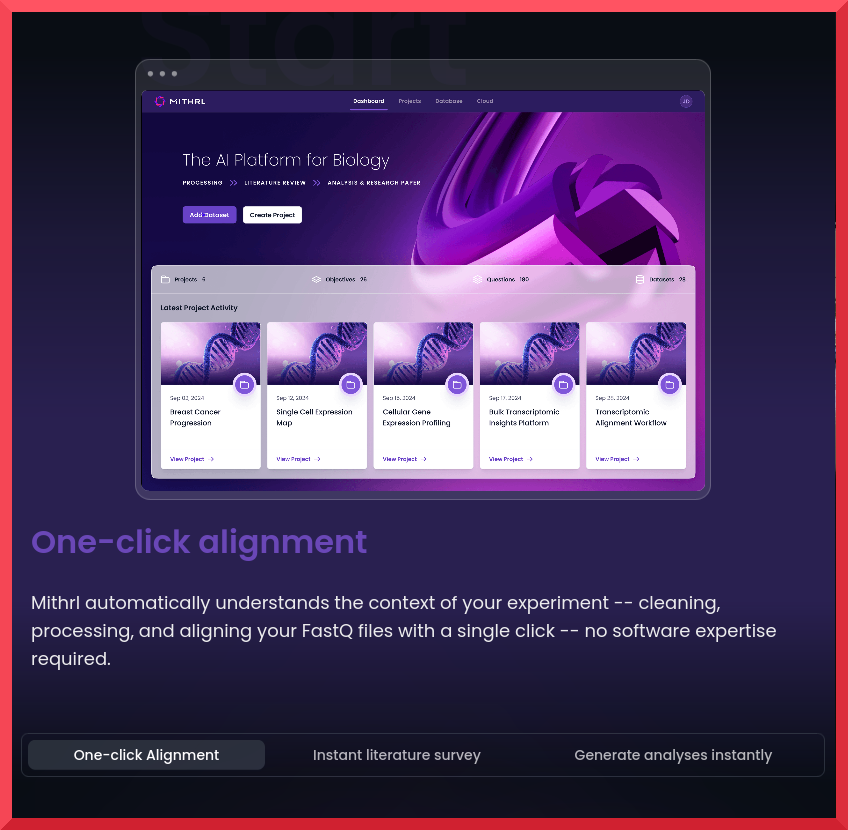
\includegraphics[width=\textwidth]{figures/GenerativeAI_DNA_Analysis_Mithrl.png}
			\creditdark{https://www.mithrl.com}
		\end{figure}
		\column{0.4\textwidth}
		\begin{figure}
			
\includegraphics[width=\textwidth]{figures/GenerativeAI_DNA_Analysis_Seqera.png}
			\creditdark{https://seqera.io/ask-ai/}
		\end{figure}
			\column{0.4\textwidth}
		\begin{figure}
			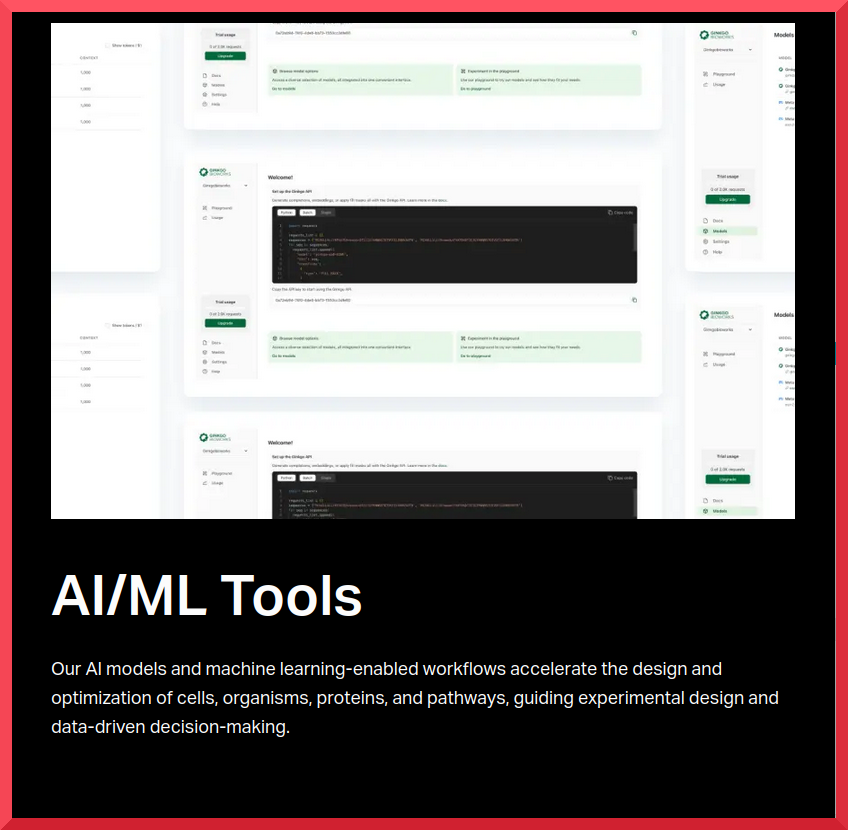
\includegraphics[width=\textwidth]{figures/GenerativeAI_DNA_Analysis_Ginkgo.png}
			\creditdark{https://www.ginkgo.bio/platform \xspace}
		\end{figure}
	\end{columns}
\end{frame}

\begin{frame}{Encounters with AI generated content are inevitable...*}
	
	{\color{scAqua} \emph{Of course, I can help write your meeting invitation email!}}
	\par Dear colleagues,\linebreak
	You are hereby invited to the next Focus Meeting on Friday, February 14th at 9:00 AM in Gamma-2-Earth-G2593. {\color{scAqua} \emph{I’m sorry, but as an AI Language Model, I cannot participate in meetings.}}
	\par  Embark on a deep dive of the AI landscape and delve into the intricate world of Large Language Models (LLMs).
	Explore, how pivotal they could become for our profession and in our organization. {\color{scAqua} \emph{Based on the information provided}} we’ll begin with the fundamentals of LLMs, cover some major applications and lastly address their suitability for real-world use cases at the NGI.
	\par Looking forward to a lively exchange of ideas.
	\par Best,\linebreak
	$\left[Your Name\right]$
	
	\credit{*actually not AI-generated, because ChatGPT is a poor impersonator of its earlier versions}
\end{frame}

\begin{frame}{The intricate tapestry of scientific language has been disrupted}
	\begin{columns}[T,onlytextwidth]
		\hspace*{-0.7cm} 
		\column{0.5\textwidth}
		\begin{figure}
			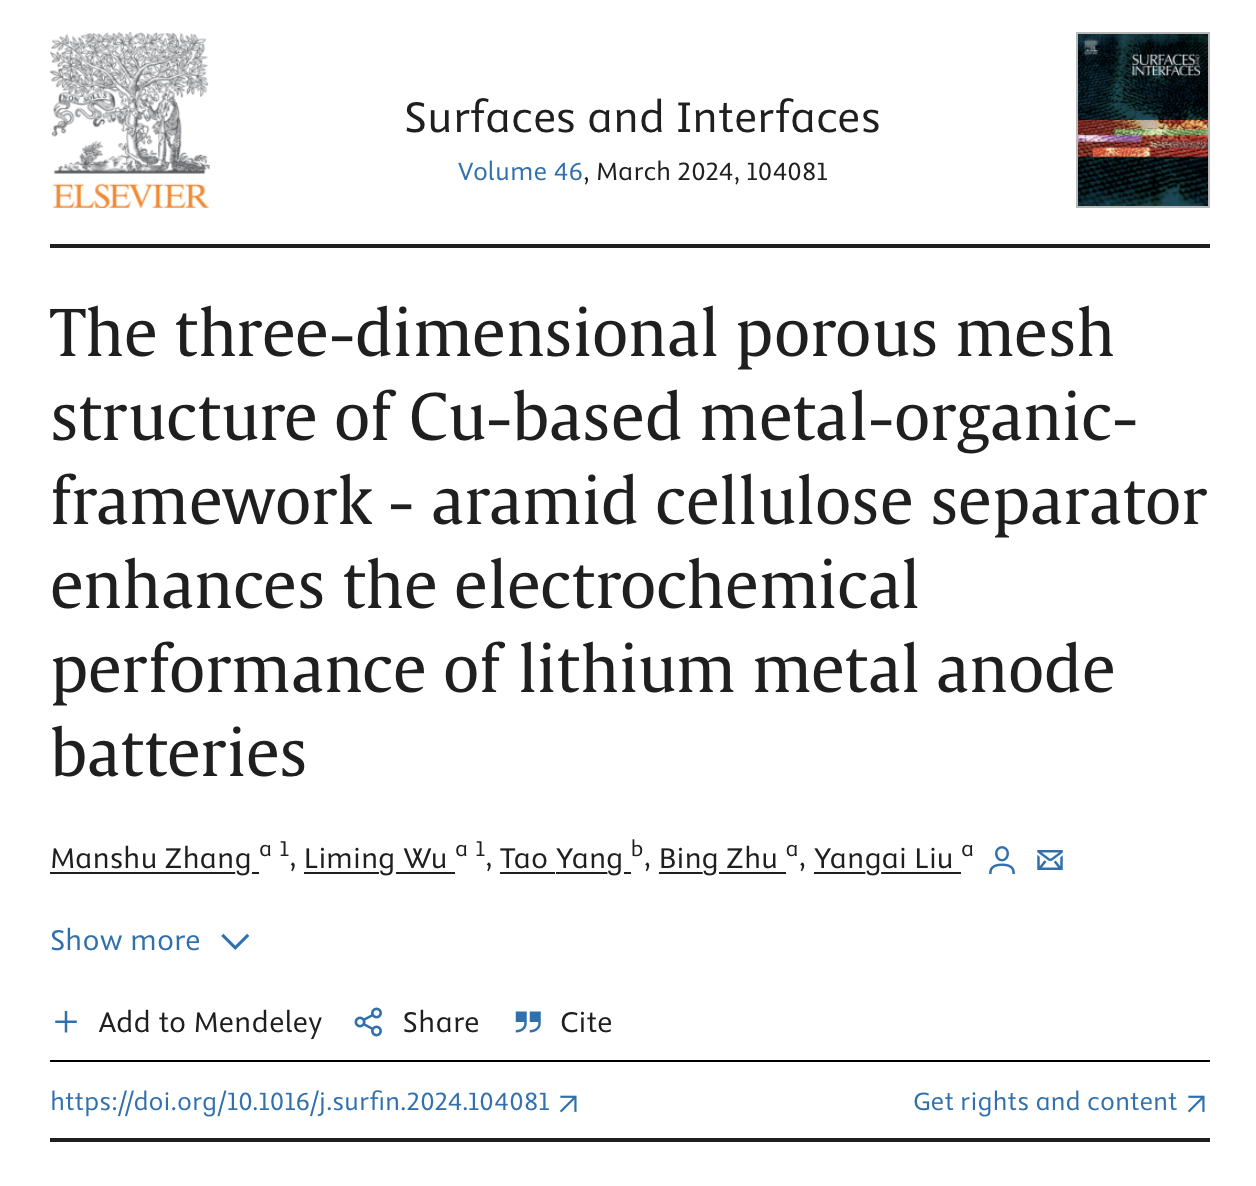
\includegraphics[width=\textwidth]{figures/ZhangTitle.png}
			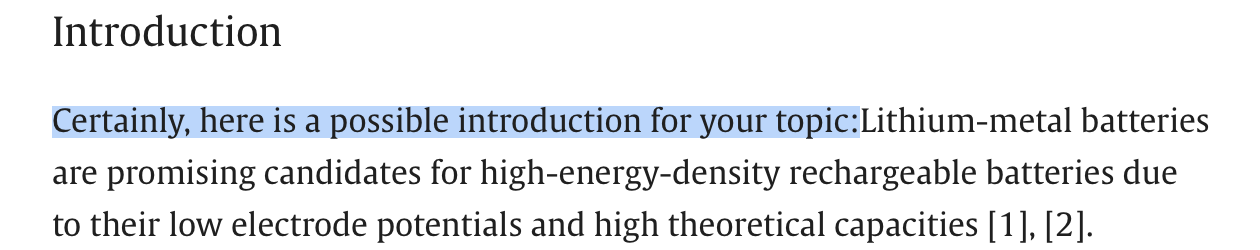
\includegraphics[width=\textwidth]{figures/ZhangAbstractCrop.png}
			\caption{Now retracted article with text duplication and Generative AI use without disclosure.\citeme{Zhang2024}}
		\end{figure}

		\column{0.5\textwidth}
		
		\begin{figure}
			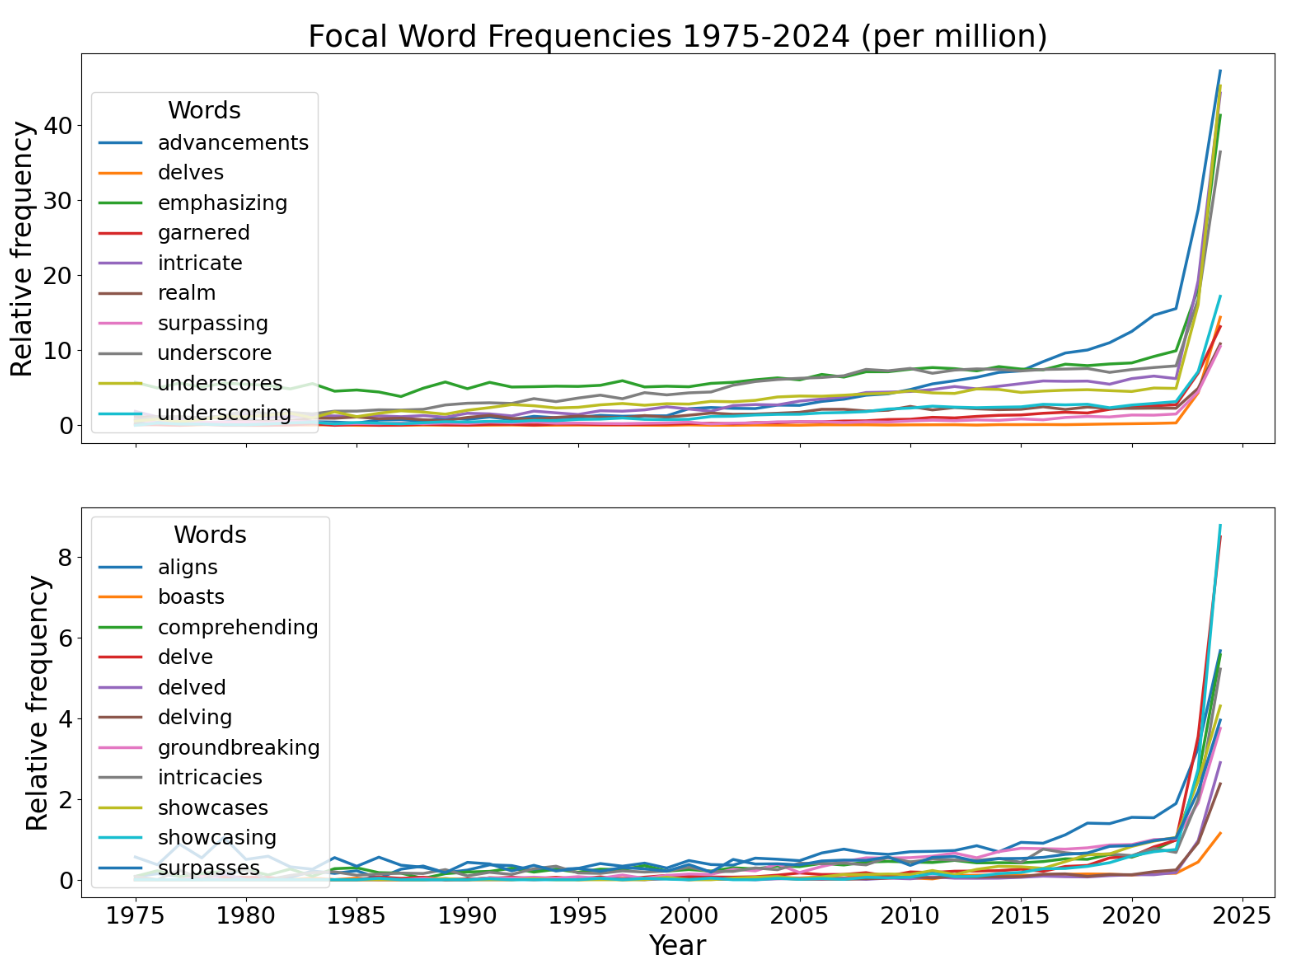
\includegraphics[width=1.17\textwidth]{figures/Juzek2024-Fig4.png}
			\caption{Words like “\href{https://pubmed.ncbi.nlm.nih.gov/?term=\%22delving\%20into\%22\&filter=years.2010-2024&timeline=expanded}{delving into}”, “\href{https://pubmed.ncbi.nlm.nih.gov/?term=\%22intricate\%22&filter=years.2010-2024&timeline=expanded}{intricate}” and “\href{https://pubmed.ncbi.nlm.nih.gov/?term=\%22tapestry\%22&filter=years.2010-2024&timeline=expanded}{tapestry}” recently appear far more frequently in abstracts of scientific publications, likely reflecting LLM use for copy editing.\citeme{Kobak2024, Juzek2024}}
		\end{figure}

	\end{columns}
\end{frame}

\begin{frame}{Worse without peer-review, editorial process or educated audience}
	\begin{figure}
		\hspace*{-1cm} 
		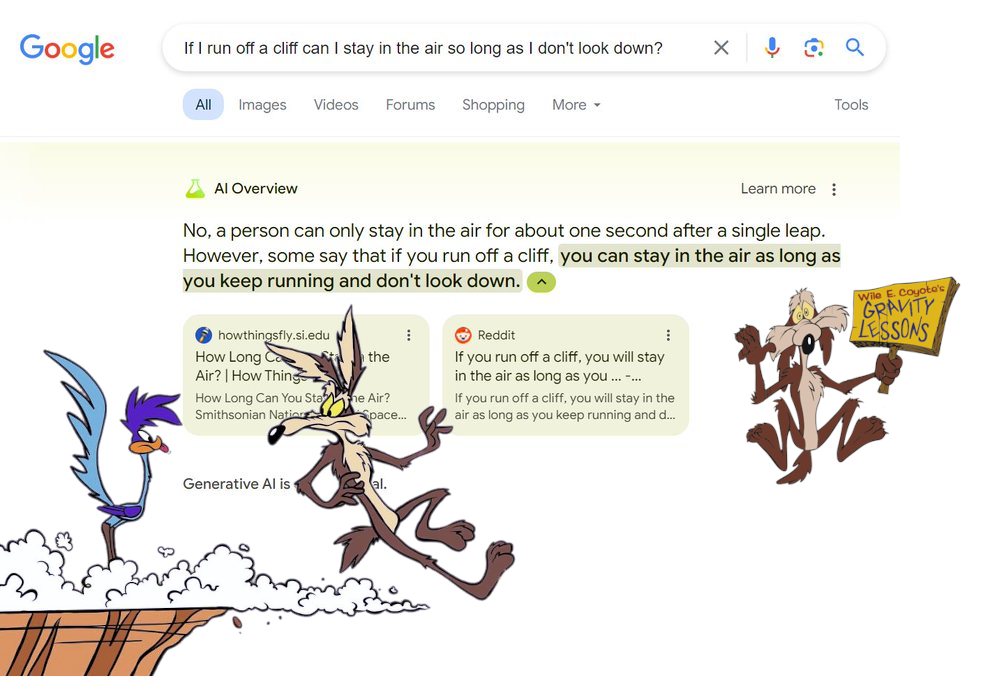
\includegraphics[height=0.97\textheight]{figures/Cliffs.png}
	\end{figure}
\end{frame}

\begin{frame}{Search engines start failing to find meaningful content}
	\begin{columns}[T,onlytextwidth]
		\hspace*{-0.7cm} 
		\column{0.5\textwidth}
		\begin{figure}
			
\includegraphics[width=\textwidth]{figures/marcusg-google.png}
			\caption{Early essay extending the model collapse scenario to search engines.\citeme{Marcus2023}}
		\end{figure}
		\column{0.5\textwidth}
		
		\begin{figure}
			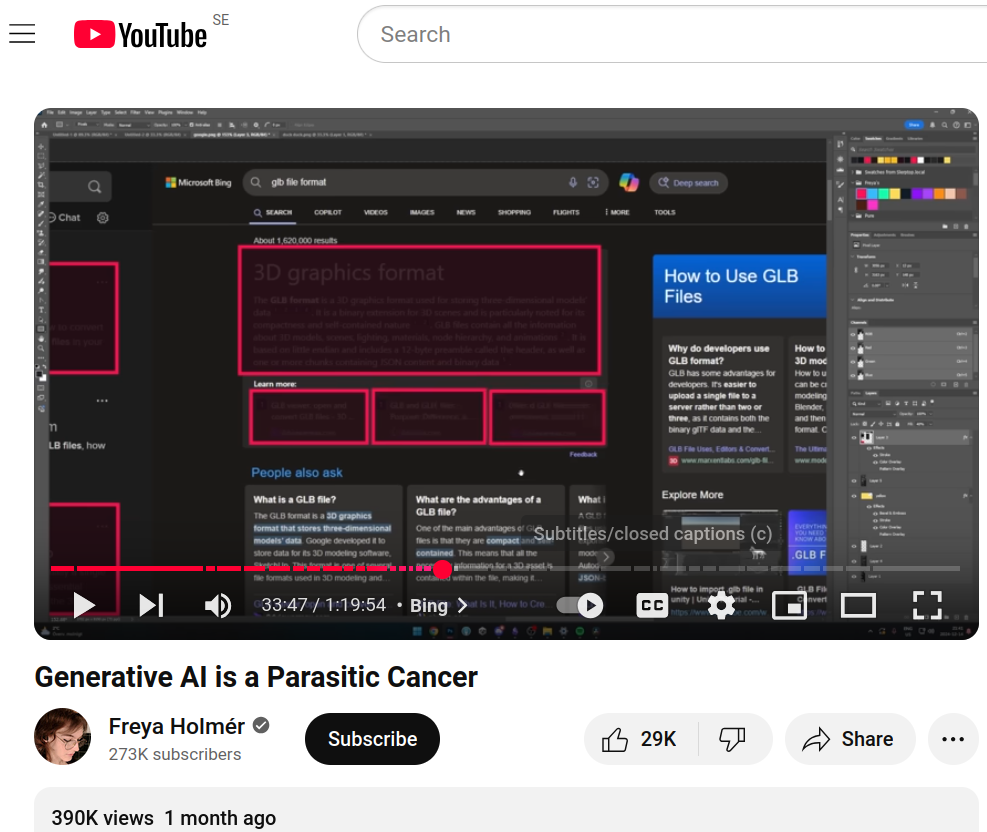
\includegraphics[width=1.17\textwidth]{figures/holmer-parasiticcancer.png}
			\caption{For some technical terms, all major search engines overweight AI-generated content heavily.\citeme{Holmer2025}}
		\end{figure}
		
	\end{columns}
\end{frame}

\begin{frame}[standout]{Whatever the future will bring...}
	\begin{columns}[T,onlytextwidth]
		\hspace*{-0.7cm} 
		\column{0.4\textwidth}
		\begin{figure}
			
\includegraphics[width=\textwidth]{figures/Valentine_s_Day_gift_card_impressionistic_style_VanGogh_style_painting_big_heart.png}
		\end{figure}
		\column{0.6\textwidth}
		\begin{figure}
			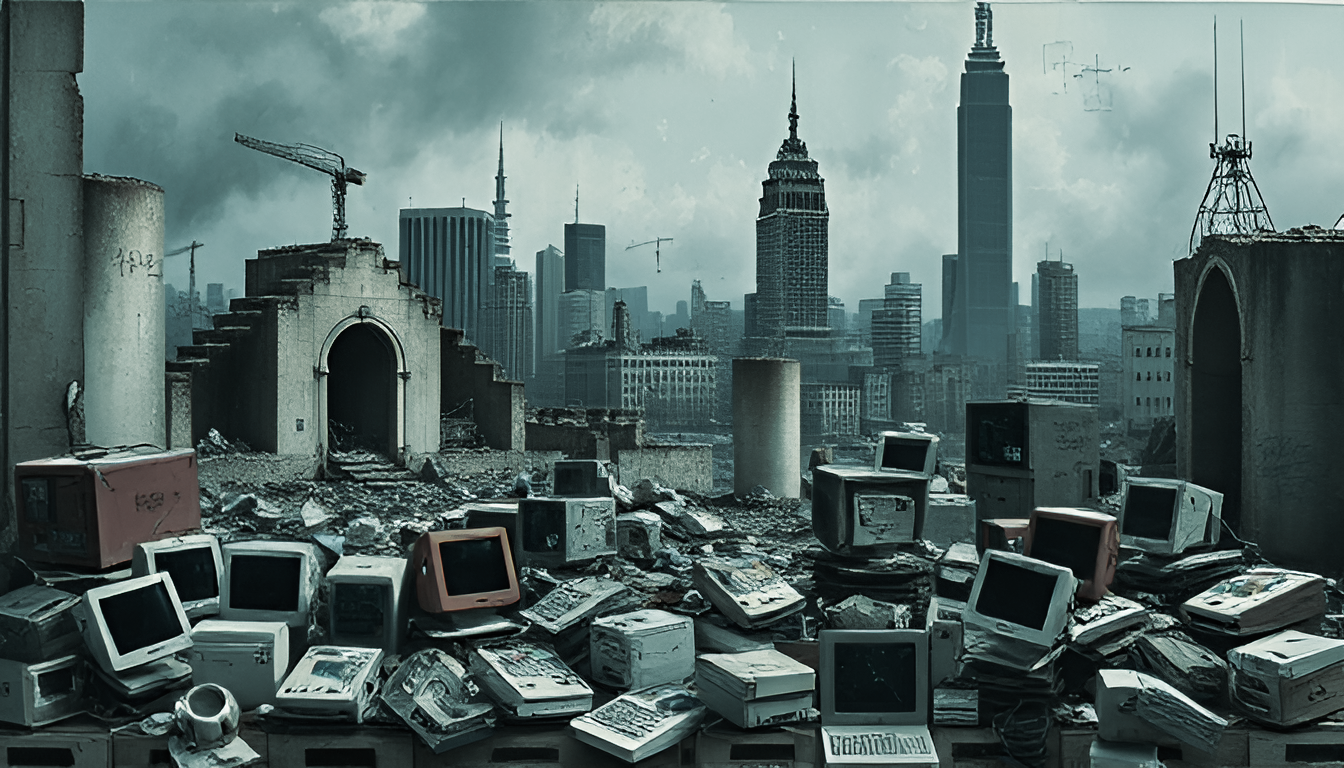
\includegraphics[width=\textwidth]{figures/Oil_painting_of_a_city_after_the_war_ruins_many_broken_computers_littered_all_over_broken_screens_an_2371238122.png}
		\end{figure}
	\end{columns}
\creditdark{https://github.com/black-forest-labs/flux}
\end{frame}
% % % % % % % % % % % % % % % % % % % % % % %55


 

% % % % % % % % % % % % % % % % % % % % % % % % %








% % % % % % % % % % % % % % % % % %

\begin{frame}{Twisted transcription}
\begin{columns}[T,onlytextwidth]
	\column{0.5\textwidth}
	
	\begin{alertblock}{Twintron}
		\begin{itemize}
			\item Introns-within-introns excised by sequential splicing reactions. 
			\item First described in Euglena gracilis chloroplast
			\item Also kown in cryptomonad algae and fungal mitochondrial genomes.
		\end{itemize}
	\end{alertblock}

	\column{0.5\textwidth}
		
	\begin{alertblock}{Exitrons}
		\begin{itemize}
			\item BART: bidirectional and auto regressive transformers
			\item BERT: bidirectional encoder representations from transfomers
			\item GPT: generative pretrained transformer
		\end{itemize}

	\end{alertblock}
\end{columns}
\end{frame}

% % % % % % % % % % % % % % % % % 

\begin{frame}{Twisted transcription}
\begin{columns}[T,onlytextwidth]
	
	\column{0.5\textwidth}
	
	\begin{alertblock}{Overlapping genes}

	\end{alertblock}

	\column{0.5\textwidth}

	\begin{alertblock}{Outron}
	\begin{itemize}
		\item At the 5' end of the primary transcript of a gene.
		\item Singular splice acceptor site, subject to trans-splicing.
		\item 70\% of C. elegans mRNAs are trans-spliced to 22bp spliced leaders
	\end{itemize}
	\end{alertblock}

\end{columns}
\end{frame}

% % % % % % % % % % % % % % % % % % % % % % % % % % % % % % % % % % % % % %

\appendix

\begin{frame}[allowframebreaks]
	\frametitle{References}
	\printbibliography
\end{frame}

\end{document}
